\documentclass{seal_thesis}

\usepackage[
  top=1.25in,
  bottom=1.25in,
  left=1.25in,
  right=1.25in
]{geometry}

\thesisType{Master Project Report}
\date{\today}
\title{GLAPP}
\subtitle{}
\author{
Fabio Isler \textmd{(09-115-965)} \\
Man Wai Li \textmd{(14-705-156)} \\
Dinesh Pothineni \textmd{(14-707-988)} \\
Riccardo Patane \textmd{(XX-XXX-XXX)}}
\home{} % Geburtsort
\country{}
\prof{Prof. Dr. Harald C. Gall}
\assistent{Dr. Philipp Leitner}
\email{}

\begin{document}
\maketitle

\abstract
Abstract


%%%%%%%%%%%%%%%%%%%%%%%%%%%%%%%%%%%%%%%%%%%%%%%%%%%%%%%%%
% NEW CHAPTER																						%
% Remember to always use a new line for a new sentence! %
%%%%%%%%%%%%%%%%%%%%%%%%%%%%%%%%%%%%%%%%%%%%%%%%%%%%%%%%%
\chapter{4 PAGES: Introduction}
\todo{DONE BY: Fabio}

Cloud computing has created a paradigm shift in the last few years, by making infrastructure available at lower costs and with higher efficiency of operations.
These solutions are increasingly being adopted by enterprises and developers, as they can provision huge amount of resources to scale on-demand in order to meet their business needs.
In cloud computing, resources such as CPU processing time, disk space, or networking capabilities, are rented and released as a service.
Today, the most important model for delivering on the cloud promise is the Infrastructure-as-a-Service (IaaS) paradigm.
In IaaS, virtual computing resources are acquired and released on demand, either via an Application Programming Interface (API) or web interface.
Along with great flexibility of being able to get new resources on demand and pay for what you use, new problems arise.
Selecting a cloud service provider can often be a quite challenging decision for the developer or a company, so is being able to monitor and evaluate these infrastructure resources on a regular basis.
With so much of variance in cost and performance, it is imperative that one would look for a reliable deployment, monitoring solutions to strike a balance with application requirements.
Furthermore, the complexity and skill required to manage multiple layers of application, data, middleware and operating systems can .

Understanding run time performance, behavior of various application components in realtime can enable us to take advantage of arbitrage opportunities that exist between different machines/regions or even other cloud providers.
For example, an application can take advantage by moving closer to its users based on timezones or traffic to improve response time.
Currently there is no flexibility to move freely between various cloud providers without great development effort and cost, however such an ability to move freely between providers enables us to benefit from cost and performance differences.
We propose a cloud middleware that can take not only take care of application deployment to cloud, but also constantly monitor and trigger such necessary adaptations to benefit from these opportunities.
Ideally this middleware also enables developers to specify their intended goals in terms of high level policies to govern the application behavior.
The middleware can then break down these policies into low level objectives, in order to trigger adaptations by changing the state of application when required.

%%%%%%%%%%%%%%%%%%%%%%%%%%%%%%%%%%%%%%%%%%%%%%%%%%%%%%%%%
% NEW SECTION																						%
%%%%%%%%%%%%%%%%%%%%%%%%%%%%%%%%%%%%%%%%%%%%%%%%%%%%%%%%%
\section{Global Living Cloud Applications}

The aim of this project is to develop a middleware for what we call ''global living cloud applications'' (GLAs).
In a nutshell, GLAs are a bio-inspired notion of cloud-native applications.
GLAs ''live'' in the cloud, and are able to migrate between data centers and cloud providers automatically, based on changes in cost and performance of cloud offerings, changes in customer behavior or requirements, or other factors.

\todo{''What I would really do is invest more thought and discussions on the conceptual model behind GLAs - I think there is something pretty cool here, but it does not seem very well-developed to me.''}


The bio-inspired terminology applies for the different levels of components of a GLA:

\begin{itemize}
	\item Cell: A cell is the lowest-level component of a GLA, consisting of the actual processes \todo{''I wonder whether it makes sense to equate cells to "processes". Is that really the same?''}
	\item Organ: An organ consists of one or more cells of the same type \todo{''For organs, I understand that organs typically also have cells of different type, i.e., an injected load balancer. I would try to make the model clear in this regard. For instance, it may make sense to distinguish between cells that are user-defined and those that come from your middleware.''}
	\item GLA: The GLA itself is a collection of organs that form the whole application
\end{itemize}

In order to manage these GLAs, we introduce a middleware called GLAPP (Global Living Application Platform).
It allows a developer to deploy multiple GLAs on whatever cloud he/she has access to and sets a centralized mechanism in place to constantly monitor and manage all the GLAs.
The middleware supports heterogeneous environment a GLA can live and move across different providers, regions, instance types, etc.
GLAPP is an open source middleware to be used on a private/individual basis.
This means that in order to be able to deploy a GLA through GLAPP, it is first required to install the GLAPP platform on the own infrastructure.
But no matter where the platform is installed, all GLAs will live in the cloud.


%%%%%%%%%%%%%%%%%%%%%%%%%%%%%%%%%%%%%%%%%%%%%%%%%%%%%%%%%
% NEW CHAPTER																						%
% Remember to always use a new line for a new sentence! %
%%%%%%%%%%%%%%%%%%%%%%%%%%%%%%%%%%%%%%%%%%%%%%%%%%%%%%%%%
\chapter{6 PAGES: Background \& Architecture}

%%%%%%%%%%%%%%%%%%%%%%%%%%%%%%%%%%%%%%%%%%%%%%%%%%%%%%%%%
% NEW SECTION																						%
%%%%%%%%%%%%%%%%%%%%%%%%%%%%%%%%%%%%%%%%%%%%%%%%%%%%%%%%%
\section{Basic Design Decisions}
\todo{IN CHARGE: Adrian}

\subsection{Main Components: Provisioning Backend, Frontend, MAPE}
\todo{Describe the design decisions of the main components}

\subsection{Deployment: Containerization with Docker}
\subsubsection{Containerization vs. other virtualization methods:}
\todo{Explain the advantage of containerization compared to e.g. virtual machines}
\subsubsection{Docker vs. other containerization implementations:}
\todo{Explain the advantage of Docker compared to e.g. OpenVZ}

\subsection{Orchestration: Docker Swarm}
\todo{Explain the advantage of Docker Swarm compared to e.g. Kubernetes}

\subsection{Rule-Based Adaptations vs. Markov Decision Process}
\todo{DONE BY: Adrian / Riccardo}
\todo{Explain the thought process behind this decision}


%%%%%%%%%%%%%%%%%%%%%%%%%%%%%%%%%%%%%%%%%%%%%%%%%%%%%%%%%
% NEW SECTION																						%
%%%%%%%%%%%%%%%%%%%%%%%%%%%%%%%%%%%%%%%%%%%%%%%%%%%%%%%%%
\section{Implementation Decisions}
\subsection{Backend: Node.js}
\todo{DONE BY: Fabio}
\todo{Explain the choice and alternatives}

\subsection{GUI: AngularJS}
\todo{DONE BY: Dinesh}
\todo{Explain the choice and alternatives}

\subsection{MAPE: Java}
\todo{DONE BY: Adrian / Riccardo}
\todo{Explain the choice and alternatives}

%%%%%%%%%%%%%%%%%%%%%%%%%%%%%%%%%%%%%%%%%%%%%%%%%%%%%%%%%
% NEW SECTION																						%
%%%%%%%%%%%%%%%%%%%%%%%%%%%%%%%%%%%%%%%%%%%%%%%%%%%%%%%%%
\section{Architecture}
The platform consists of 3 different parts/blocks: a front end, a provisioning component and a control loop.
The front end provides an interface for developer to interact with the middleware to deploy and manage his/her GLAs.
The provisioning component provides the management functionalities of the middleware including cloud infrastructure management, application deployment and access to the application status information.
Lastly the control loop is the component responsible for enabling the management of GLAs by the middleware itself.
It follows the MAPE (Monitoring, Analysis, Planning and Execution) principle.
Possible execution actions are moving cells between different cloud instances (migration), duplicating/splitting cells of the GLA (mitosis), or removing cells.

\begin{figure}[!ht]
\centering
	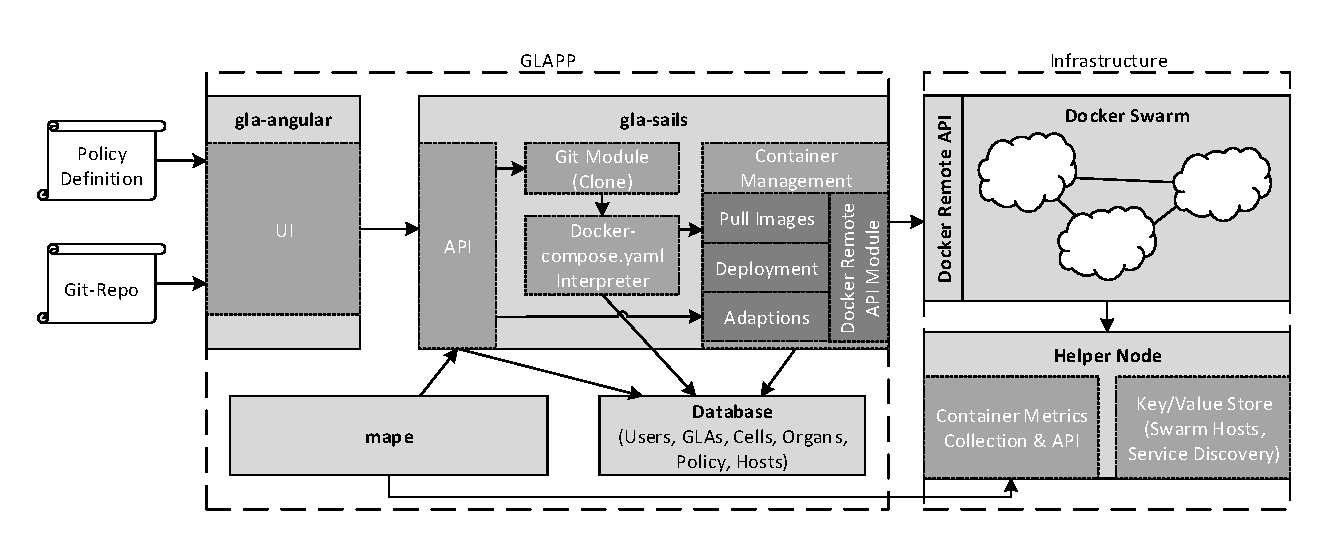
\includegraphics[width=\textwidth]{detailed_architecture.pdf}
	\caption{Detailed Architecture of GLAPP and the Infrastructure}
	\label{fig:detailed}
\end{figure}
\todo{Explain the separate parts - DONE BY: Dinesh}

\noindent\todo{''I like Fig2 better, but there is still plenty of room for improvement. For instance, I would remove the word "optimal" from the figure - especially, if we now use this iterative Q-learning approach, our deployment will often *not* be optimal, at least temporarily. I am also quite suspicious that the msot dominant block in the figure is the provisioner. Is this really what we want to emphasize?''}


%%%%%%%%%%%%%%%%%%%%%%%%%%%%%%%%%%%%%%%%%%%%%%%%%%%%%%%%%
% NEW CHAPTER																						%
% Remember to always use a new line for a new sentence! %
%%%%%%%%%%%%%%%%%%%%%%%%%%%%%%%%%%%%%%%%%%%%%%%%%%%%%%%%%
\chapter{10 PAGES: Components}

%%%%%%%%%%%%%%%%%%%%%%%%%%%%%%%%%%%%%%%%%%%%%%%%%%%%%%%%%
% NEW SECTION																						%
%%%%%%%%%%%%%%%%%%%%%%%%%%%%%%%%%%%%%%%%%%%%%%%%%%%%%%%%%
\section{3 PAGES: Backend}
\todo{DONE BY: Fabio}


%%%%%%%%%%%%%%%%%%%%%%%%%%%%%%%%%%%%%%%%%%%%%%%%%%%%%%%%%
% NEW SECTION																						%
%%%%%%%%%%%%%%%%%%%%%%%%%%%%%%%%%%%%%%%%%%%%%%%%%%%%%%%%%
\section{2 PAGES: GUI}
\todo{DONE BY: Dinesh}


%%%%%%%%%%%%%%%%%%%%%%%%%%%%%%%%%%%%%%%%%%%%%%%%%%%%%%%%%
% NEW SECTION																						%
%%%%%%%%%%%%%%%%%%%%%%%%%%%%%%%%%%%%%%%%%%%%%%%%%%%%%%%%%
\section{4 PAGES: MAPE}
\todo{DONE BY: Adrian / Riccardo}
Being the control loop of the whole platform, MAPE interfaces with SAILS to retrieve environment information, with monitoring system to retrieve performance metrics, perform computation within itself to decide adaptation action and, in the end, communicate to SAILS to execute the adaptation action.

Regarding the interface with SAILS and monitoring system, HTTP protocol is used with JSON objects in the request and response.
The use of JSON objects allows an data structure that is flexible to represent different types of information and to facilitate data exchange.
The information retrieved from SAILS includes the infrastructure information of virtual machines, deployment information of application components and their underlying containers.
It also includes user-defined policy from the database as well as performance metrics from the backend monitoring system.

Prometheus \todo{add reference} is a monitoring system that can provide both infrastructure and application performance metrics.
Infrastructure metrics are provided by exporters, which is a set of library that expose metrics data of the host environments and the Docker containers.
Application metrics are provided with the use of custom-built program to expose the needed data in a Prometheus exposition format \todo{add reference}.
The use of Prometheus and its exposition format enable MAPE to access custom metrics such as application performance data or cost metrics of the host from various cloud service providers.

% computation of healthiness values
\todo{elaborate about healthiness computation}

% range query and point query in Prometheus
Prometheus is also sophisticated in providing different types of query.
It supports range query and point query with additional functions that can be applied on the raw data when formulating a query.
This enables the fine-grained extraction of data that best fits the corresponding performance metric.
For instance, the rate function allows the direct retrieval of the rate of change in CPU time of a container with configurable data point range, data point interval and duration covered by each data point.
The robust query functionality provides two major advantages.
First of all, it reduces the complexity of computation logic of MAPE that is responsible for getting specific performance metric for subsequent healthiness computation.
Secondly, it allows quick tweaking of query parameters to obtain the most relevant data for adaptation action determination during later development stage. 

% burlap library for MDP and its extensibility
After the healthiness values of the each individual cell is computed based on the policy and performance metric, all violating cells within an organ are taken into account for an evaluation.
When the number of violating cell exceed a defined threshold, the organ will be considered as unhealthy.
Once an organ is unhealthy, information of all violations will be further processed in MAPE to determine appropriate adaption action.

% rule based adaptation vs MDP



%%%%%%%%%%%%%%%%%%%%%%%%%%%%%%%%%%%%%%%%%%%%%%%%%%%%%%%%%
% NEW SECTION																						%
%%%%%%%%%%%%%%%%%%%%%%%%%%%%%%%%%%%%%%%%%%%%%%%%%%%%%%%%%
\section{2 PAGES: Other}
\subsection{Monitoring / Prometheus}
\todo{DONE BY: Adrian / Riccardo}

\subsection{Supporting Applications}
\todo{Infrastructure Scripts, Consul, Registrator, Voting-App, Proxy, metrics-server etc.}
\todo{DONE BY: Fabio}



%%%%%%%%%%%%%%%%%%%%%%%%%%%%%%%%%%%%%%%%%%%%%%%%%%%%%%%%%
% NEW CHAPTER																						%
% Remember to always use a new line for a new sentence! %
%%%%%%%%%%%%%%%%%%%%%%%%%%%%%%%%%%%%%%%%%%%%%%%%%%%%%%%%%
\chapter{7 PAGES: Case Study}
\todo{DONE BY: Riccardo}

\section{Explain Demo Application}
\begin{itemize}
	\item Explain concept of the app at high level
	\item Explain the components themselves
	\item Explain the docker-compose file
	\item Explain our custom metrics (costs, clicks)
	\item Explain modifications to the app (region switch button, POST request with click-origin to metrics-server with every click
\end{itemize}

\section{Scenarios}
\begin{itemize}
	\item Explain the scenarios
	\item Explain the triggers
	\item Explain how MAPE realizes a necessary adaptation
\end{itemize}


%%%%%%%%%%%%%%%%%%%%%%%%%%%%%%%%%%%%%%%%%%%%%%%%%%%%%%%%%
% NEW CHAPTER																						%
% Remember to always use a new line for a new sentence! %
%%%%%%%%%%%%%%%%%%%%%%%%%%%%%%%%%%%%%%%%%%%%%%%%%%%%%%%%%
\chapter{2 PAGES: Future Work}
\todo{DONE BY: Fabio / Adrian}



%%%%%%%%%%%%%%%%%%%%%%%%%%%%%%%%%%%%%%%%%%%%%%%%%%%%%%%%%
% NEW CHAPTER																						%
% Remember to always use a new line for a new sentence! %
%%%%%%%%%%%%%%%%%%%%%%%%%%%%%%%%%%%%%%%%%%%%%%%%%%%%%%%%%
\chapter{1 PAGE: Conclusion}


\bibliographystyle{alpha}
\bibliography{sources}

%%%%%%%%%%%%%%%%%%%%%%%%%%%%%%%%%%%%%%%%%%%%%%%%%%%%%%%%%
% NEW CHAPTER																						%
% Evt. APPENDIX
% Remember to always use a new line for a new sentence! %
%%%%%%%%%%%%%%%%%%%%%%%%%%%%%%%%%%%%%%%%%%%%%%%%%%%%%%%%%


\end{document}
